\documentclass[11pt,a4paper]{article}

\usepackage[utf8]{inputenc}
\usepackage[T1]{fontenc}
\usepackage{lmodern}
\usepackage[french]{babel}
\usepackage[margin=2.1cm]{geometry}
\usepackage{microtype}
\usepackage{amsmath,amssymb}
\usepackage{booktabs}
\usepackage{array}
\usepackage[table]{xcolor}
\usepackage{graphicx}
\usepackage{caption}
\usepackage[most]{tcolorbox}

\definecolor{navy}{HTML}{1F3864}
\definecolor{bluemid}{HTML}{2E5496}
\definecolor{lightblue}{HTML}{D6E0F0}

\captionsetup{font=small,labelfont={bf,color=navy},labelsep=period}
\graphicspath{{../figures/}}

\newtcolorbox{cle}[1][]{colback=lightblue!40,colframe=navy,boxrule=0.6pt,
  arc=2pt,left=8pt,right=8pt,top=6pt,bottom=6pt,#1}

\title{\vspace{-1.2cm}\color{navy}\bfseries La décomposition $W=S+A$ comme réversibilité d'un processus\\[2pt]
  \large Le parallèle avec la martingalisation, et sa faisabilité}
\author{Kélian Kaddouri}
\date{27 juillet 2026}

\begin{document}
\maketitle
\vspace{-0.9cm}

\begin{cle}
\textbf{La question de Hugo.} La décomposition d'une matrice en partie symétrique
$S=(W+W^{\top})/2$ et antisymétrique $A=(W-W^{\top})/2$ est-elle le miroir de la
décomposition d'un processus stochastique en une partie martingale et sa dérive, et ce
parallèle est-il \emph{faisable}~? Réponse~: oui, et il ne fait pas qu'illustrer, il
\textbf{fonde} la limite d'identification du mémoire sur un théorème standard, au lieu de
la constater. Ce que le script~32 pose comme fait algébrique (la donnée voit $S$, pas
$A$), la théorie des processus réversibles le rend nécessaire.
\end{cle}

\medskip
\noindent\textbf{Le dispositif.} On construit sur les cinq piliers la chaîne de Markov qui
saute de $i$ vers $j$ proportionnellement au jugement dirigé, $P_{ij}=\mathrm{TRANS}[i][j]
/\sum_j \mathrm{TRANS}[i][j]$. Elle porte exactement la direction posée. Soit $\pi$ sa loi
stationnaire. Le renversement du temps donne la chaîne adjointe $\tilde P_{ij}=\pi_j P_{ji}
/\pi_i$, d'où
\[
  P = S + A, \qquad S=\tfrac12(P+\tilde P)\ \text{(réversible)}, \qquad
  A=\tfrac12(P-\tilde P)\ \text{(courant)},
\]
et sous renversement $S$ est invariante tandis que $A$ change de signe. C'est le miroir
exact de $S$ et $A$ du mémoire~: $S$ est la co-occurrence, symétrique au sens du temps~;
$A$ est la direction, ce qui distingue l'avant de l'après.

\medskip
\begin{center}
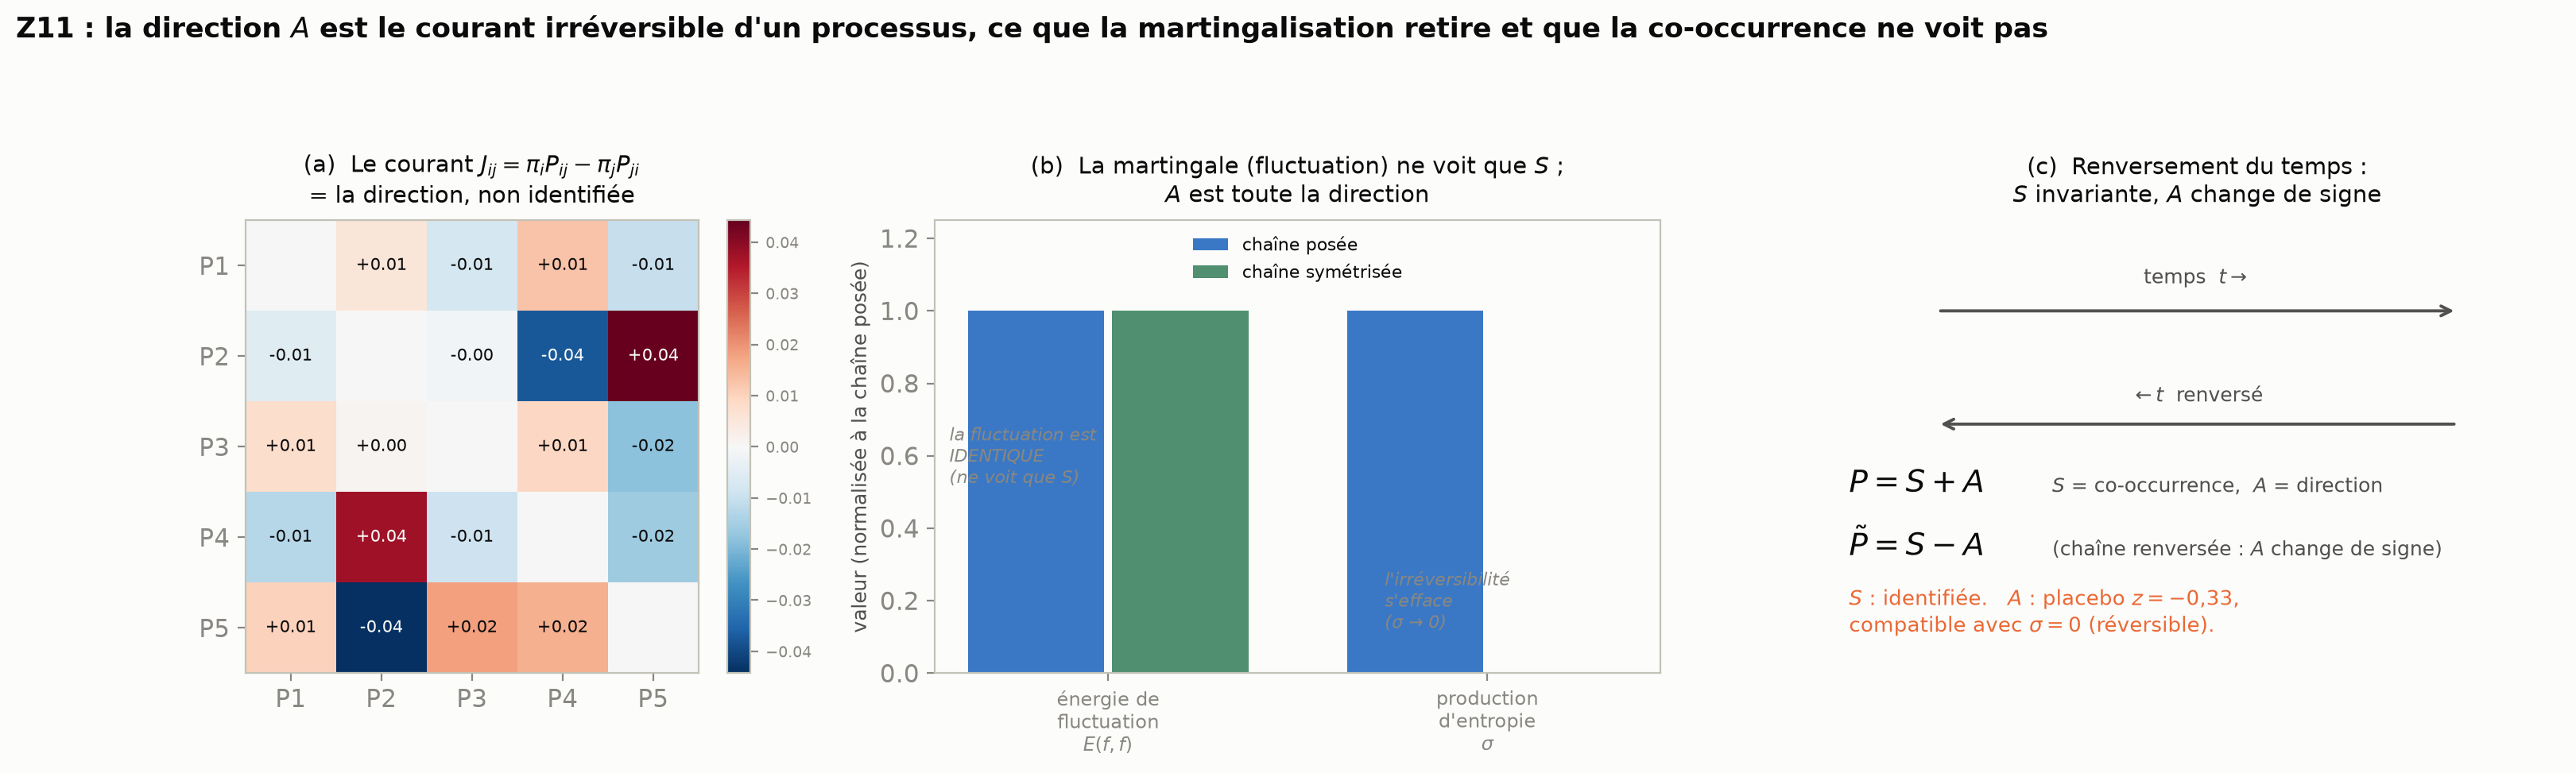
\includegraphics[width=\linewidth]{Z11_reversibilite_martingale.png}
\captionof{figure}{Trois identités vérifiées numériquement (script~40). \textbf{(a)} le
courant $J_{ij}=\pi_iP_{ij}-\pi_jP_{ji}$ est non nul ($\max|J|=0{,}044$)~: le modèle porte
une direction. \textbf{(b)} l'énergie de fluctuation (forme de Dirichlet, la variation de la
martingale) est \emph{identique} pour la chaîne posée et sa symétrisée, alors que la
production d'entropie $\sigma$ s'efface à la symétrisation. \textbf{(c)} le renversement du
temps laisse $S$ intacte et retourne $A$.}
\end{center}

\begin{cle}
\textbf{Les trois identités, en clair.}
\begin{enumerate}\itemsep2pt
\item \textbf{Courant et réversibilité.} La chaîne est réversible (équilibre détaillé) si
et seulement si le courant $J=0$. Ici $\max|J|=0{,}044>0$~: irréversible, donc dirigée.
\item \textbf{La fluctuation ne voit que $S$ (la martingalisation).} Pour toute fonction
test $f$, la forme de Dirichlet $E(f,f)=\tfrac12\sum_{ij}\pi_iP_{ij}(f_j-f_i)^2$ ne dépend
\emph{que} de la partie réversible~: $E_P(f,f)=E_{S}(f,f)$ à $10^{-15}$ près, la part
antisymétrique $A$ y contribue exactement $0$. La martingale (la fluctuation) est aveugle
à la direction~; seule la dérive, le compensateur, la porte. C'est précisément ce que la
martingalisation retire.
\item \textbf{La direction $=$ production d'entropie.} L'irréversibilité tient dans un seul
scalaire, $\sigma=\tfrac12\sum(\pi_iP_{ij}-\pi_jP_{ji})\log\frac{\pi_iP_{ij}}{\pi_jP_{ji}}
\ge 0$, nul ssi réversible. On mesure $\sigma=0{,}070$ pour la chaîne posée, $\approx
5\times10^{-33}$ pour la symétrisée.
\end{enumerate}
\end{cle}

\medskip
\noindent\textbf{Ce que le parallèle apporte au placebo.} Le test directionnel du mémoire
(asymétrie observée $119$ sous le nul de permutation $128\pm27$, $z=-0{,}33$) ne se lit plus
comme un échec de calibration mais comme un test de $\sigma=0$~: la co-occurrence observée
est \textbf{compatible avec une dynamique réversible}. La limite devient une limite de
principe. Une statistique invariante par renversement du temps ne peut pas identifier un
courant qui, lui, change de signe sous ce renversement. C'est le même énoncé que la
proposition~3 du script~32 ($W$ et $W^{\top}$ observationnellement indistinguables), mais
adossé au théorème plutôt qu'au calcul isolé.

\begin{cle}[colback=orange!8,colframe=orange!70!black]
\textbf{Honnêteté (esprit Vasicheck).} Deux réserves à assumer explicitement.
\textbf{(i)} La version propre du courant est pondérée par $\pi$ (produit scalaire de
$L^2(\pi)$)~; le $S=(W+W^{\top})/2$ du mémoire en est le cas particulier $\pi$ uniforme. Ici
l'écart est faible ($\max_i|\pi_i-1/5|=0{,}069$), donc les deux lectures coïncident en
pratique, mais la version pondérée est la forme correcte. \textbf{(ii)} $W$ est un noyau de
contagion, pas littéralement un générateur de Markov~: on \emph{emprunte} l'algèbre de la
réversibilité comme analogie éclairante, on ne pose pas que la cascade \emph{est} une chaîne
réversible. C'est une lecture, pas une hypothèse de plus.
\end{cle}

\smallskip
\noindent\footnotesize\textcolor{navy}{\textbf{Source.}} Script
\texttt{6\_contagion/40\_reversibilite\_martingale.py}, figure
\texttt{Z11\_reversibilite\_martingale.png}. Prolonge le script~32 (propriétés formelles,
proposition~3) et le module \texttt{partial\_id}. Part antisymétrique euclidienne
$\lVert A\rVert/\lVert W\rVert=40{,}7\,\%$.

\end{document}
